\begin{task}[
  title=Astronomy application,
  id=astro,
  lead=CDS,
  PM=18,
  wphases={0-48},
  partners={QS,WTT,SRL,INSERM,XFEL}
]

  Context: The Strasbourg Astronomical Data Center (CDS) is scientific data 
  center hosted by the Observatory of Strasbourg. The CDS plays a unique and 
  essential role in astronomy by adding value to published and reference data. 
  CDS runs astronomical services that
  provide data for the world-wide astronomy research community. Its three main
  services (SIMBAD, VizieR and Aladin) are heavily used with up to one million
  queries per day.  These services be accessed through web interfaces, mainly
  for human interaction, as well as through programmatic interfaces, including
  the standardized protocols defined by the International Virtual Observatory
  Alliance.

  Python and notebooks are rapidly increasing in importance for astronomy 
  research. Indeed, Python for Astronomy software ecosystem has known a 
  constant steady growth in the latest years, as shown in 
  figure~\ref{fig:python-astro-citations}.


  We will develop a Jupyter-based framework to efficiently access, explore,
  visualize and analyze reference data that are available through CDS services 
  as a real example of using open astronomy data.
  We will provide scientific users with a set of customizable Jupyter notebooks
  for visualization and analysis tasks, providing a new level of
  interoperability with python libraries and notebooks as is highly demanded
  by the astronomy research community.

  The focus is on the two following user stories:
    \begin{compactitem}
        \item analysis of catalogue data results, up to billions of rows.
              Tabular data is the typical output of SIMBAD and VizieR data.
        \item modular dashboard-like interface providing a top level
              interactive view of the available data for a given astronomical
              object and enabling loading and analysis of those data.
    \end{compactitem}


  This task will build on existing Python libraries to access CDS data
  (\textit{astroquery.[cds/simbad/vizier/xmatch]}). For visualization, we will 
  use proven tools like \textit{GLUE} and \textit{ipyvolume}, which are now 
  built upon the Jupyter stack.
  We will also make significant improvement to existing Jupyter widgets 
  (\textit{ipyaladin}, interactive sky atlas running in the notebook) and 
  develop a new widget to offer a tree-like view of available datasets.

  We will also develop Python libraries to allow integration and usage in
  notebook of existing CDS infrastructure services, namely CDSLogin (which
  provides authentication) and CDS MyData (remote storage space for tabular
  data).
  This will allow the user to interact with one's personal storage space from
  the notebook. It will also allow for advanced customisation of the interface 
  to fit user needs.

  The work is organised with a 2 stage approach. Firstly, the generated 
  notebooks will run locally on user machines (representing a milestone for 
  this task). Following the Binder development in \WPref{eosc}, we will aim 
  to run these notebooks on the European Binder Service. The aspiration is 
  that this contributes to the development of innovative services for the EOSC.
  The deliverable of this task will be a demonstrator available to the 
  scientific user community (\localdelivref{application-astro}).

  Milestone 4.X: Astronomical data services based on reference astronomy data from CDS are made available in jupyter notebooks, and decision point on how to use developments of WP5 for running these notebooks on the European Binder Service.

\TODO{how to formally describe the milestone??}


  Access to the notebooks will be provided as a one-click action option from
  SIMBAD and VizieR results pages.
  Thus, providing with a one-click way of visualizing, filtering and analyzing
these potentially large tables will bridge the gap between access and analysis
of the data, with zero installation for the user.
  For specific science cases, we will explore rendering of notebooks with 
  interactive widgets through "Voila", as to allow users not familiar with 
  Python to benefit from the Jupyter notebook framework.

  These new developments will be highly visible to the large number of astronomers who use the CDS services (50,000 unique visitors per month) and such tools are in high demand by these users.

  The CDS expertise in astronomy data and interfaces will be profitably combined with expertise of BOSSEE partners to ensure the deployment of high quality widgets (Simula, WildTree Tech, QuantStack).


\begin{figure}[ht]\centering
  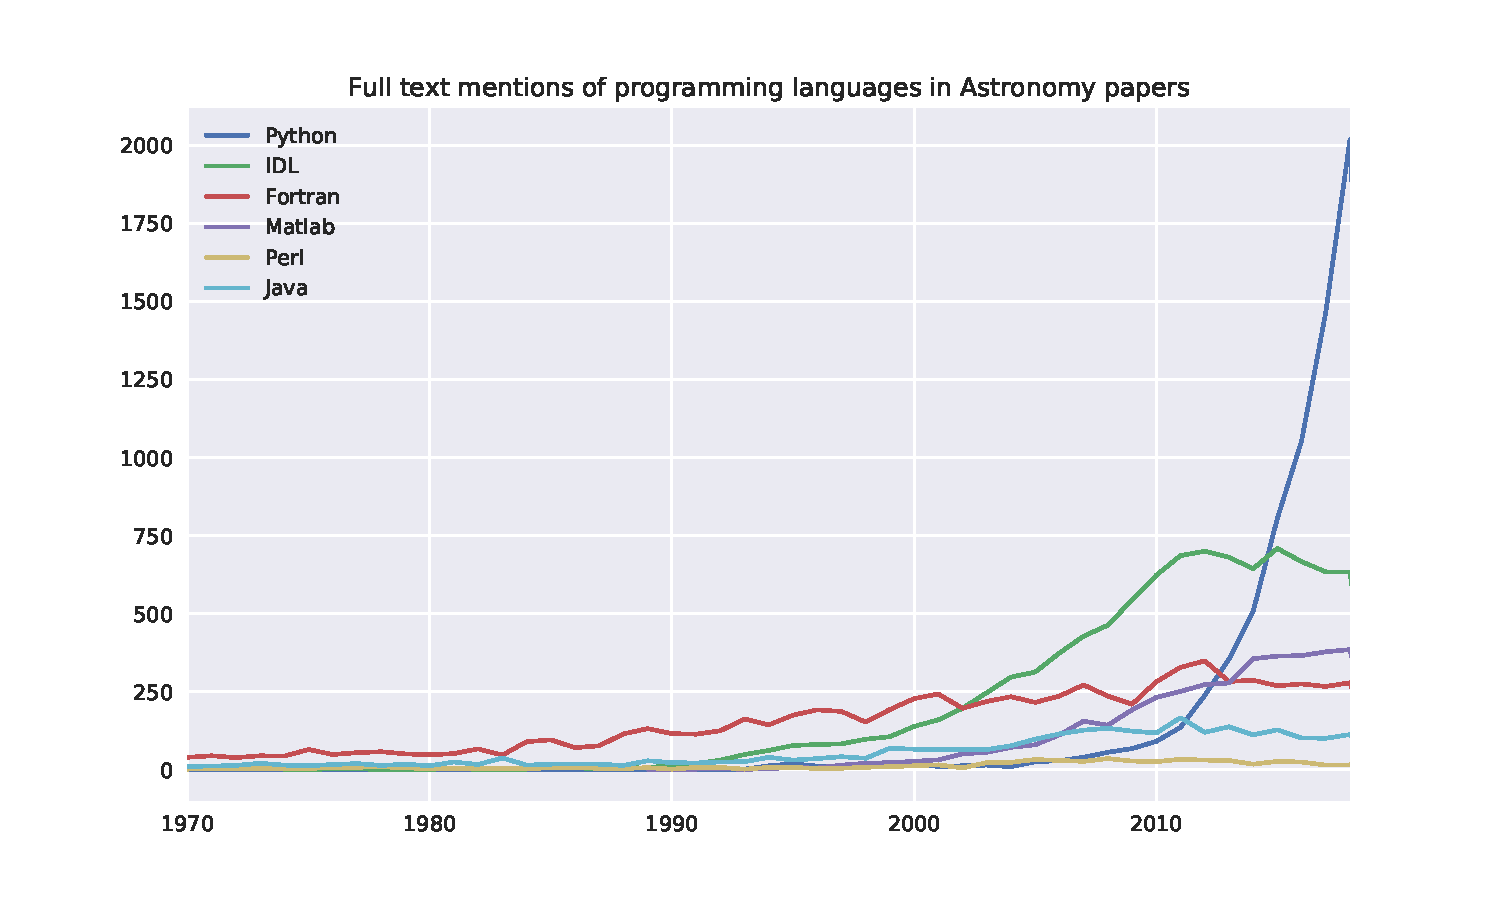
\includegraphics[width=0.8\textwidth]{python-astro-citations}
  \caption{Mentions of programming languages in refereed Astronomy papers, extracted from ADS. Python usage has increased dramatically in the recent years.}\label{fig:python-astro-citations}
\end{figure}

Deliverable: \localdelivref{application-astro}


\end{task}
